\subsection{Time walk corrlection of CDC}
Start timing of CDC was of cause depend on the velocity of decay particle because reach time to drift area was depend on the velocity.
Actually, the correlation between residual of CDC and the $1/\beta^2$ was seen in Fig\ref{fig:CDC_ob2_res}.
The correlation was collected using time-walk collection like method by fitting with following function
\begin{equation}
  t_{corrected}=p_0+p_1 \beta+p_2\beta^2+p_3\exp(p_4\beta).
\end{equation}
This collection was adopted wire-by-wire of the CDC.
Fig\ref{fig:CDC_ob2_res} represents all wire summed scatter plot.
The figure after collection (right) seen almost no correlation.

\begin{figure}[htbp]
  \centering
  \begin{tabular}{cc}
    \begin{minipage}{0.5\hsize}
      \includegraphics[width=5cm]{../pic/Run78/CDS/CDC_ob2_res.eps}
    \end{minipage}
    \begin{minipage}{0.5\hsize}
      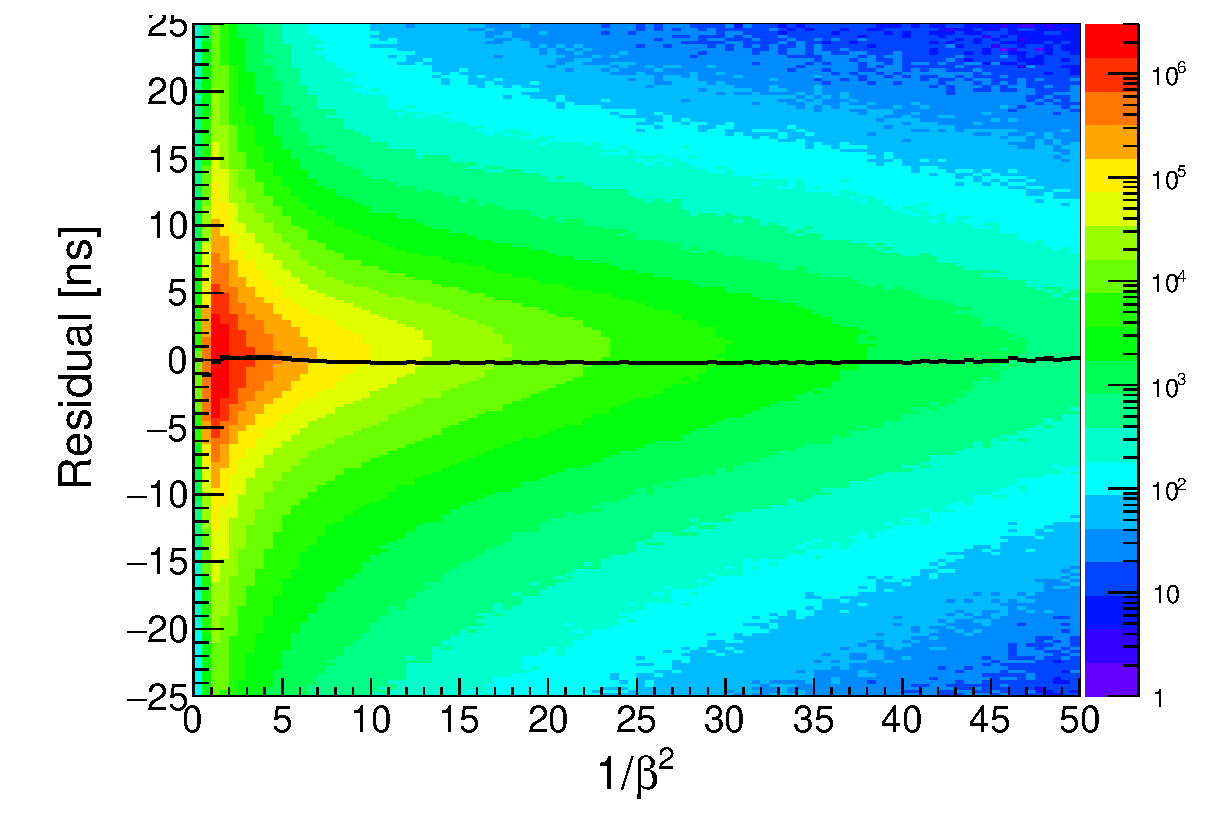
\includegraphics[width=5cm]{../pic/Run78/CDS/CDC_ob2_res_after.eps}
    \end{minipage}
  \end{tabular}
  \caption{
    These figures show correlation between $1/\beta^2$ and residual convert to time using dt-dx correction function.
    Left figure shows before time-walk collection.
    Right figure shows after time-walk collection.
  }
  \label{fig:CDC_ob2_res}
\end{figure}
